\documentclass[11pt]{article}
\usepackage[a4paper,margin=25mm]{geometry}
\usepackage{amsmath,amssymb,booktabs,longtable,array,graphicx}
\usepackage[T1]{fontenc}
\usepackage{url}
\usepackage{hyperref}
\urlstyle{same}
% Permit line breaks inside hexadecimal transaction identifiers as well as paths.
\makeatletter
\g@addto@macro\UrlBreaks{\do\a\do\b\do\c\do\d\do\e\do\f\do\0\do\1\do\2\do\3\do\4\do\5\do\6\do\7\do\8\do\9}
\makeatother
\setlength{\emergencystretch}{2em}
\setlength{\tabcolsep}{4pt}
\renewcommand{\arraystretch}{1.12}
\usepackage{tikz}
\usetikzlibrary{arrows.meta,positioning,fit,backgrounds}
\hypersetup{colorlinks=true,urlcolor=blue,citecolor=blue,linkcolor=blue}
\newcommand{\code}[1]{\nolinkurl{#1}}
\title{Countersign: Transaction-Bound Agent Payments with Whitechain, World and ENSv2\\\large A systems-security implementation case study}
\author{Somesh S. Talligeri\\\small\url{https://github.com/SomeshTalligeriDEV}}
\date{7 November 2026\\\small Preprint draft: authorship confirmation and review required; not independently audited}
\begin{document}
\maketitle
\begin{abstract}
Autonomous agents need authority to request payments without acquiring unrestricted authority over a treasury. COUNTERSIGN composes three distinct mechanisms: Whitechain contracts enforce stablecoin transfers and spending policy; World sandbox authentication supplies fresh subject evidence for application-owned human approval; and ENSv2 supplies discoverable agent identity with scoped record-write permissions. None substitutes for the other. Typed payment intents bind the transfer, and threshold payments additionally require an exact owner signature and a separate authentication attestation. We specify the replay domains, policy epochs, cancellation limits and cross-chain trust boundary, then evaluate their implementation using adversarial tests and provenance-separated integration records. The current Node rerun contains 157 passing tests; the recorded Solidity checkpoint contains 131 executions, including inherited repetitions, plus three shared digest cases. Recorded public-testnet evidence includes official-USDT settlement, a sandbox-authenticated payment and ENS registry/resolver setup. These observations are not a claim of complete current-release acceptance: deployed-state ENS fork execution and fresh integrated browser verification remain incomplete, and two historical six-step runs reached five steps each. A four-case, single-sample local mock-token gas experiment is reported separately from network performance. The contribution is a systems-security composition and empirical implementation analysis, not a new cryptographic primitive, independent audit or production identity guarantee.
\end{abstract}

\section{Introduction}
Delegating a purchase to software creates two separate questions: which operations may the software propose, and which operation has a human actually authorized? A wallet key with unrestricted transfer authority collapses these questions. Server-side controls can separate them, but their force depends on whether a compromised server can move funds through another path. A signed approval can narrow authority only if the execution endpoint verifies exactly the authorized fields and consumes the authorization in an appropriate replay domain.

COUNTERSIGN is a prototype for bounded agent-initiated stablecoin payments. A treasury owner installs a spending policy and a limited token allowance. An agent signs payment intents. Payments below a configured threshold require no further interaction; payments at or above it require an owner signature over the exact intent and an attestor signature connecting that approval to fresh World authentication. The relayer pays execution gas. The agent need not hold settlement tokens or the chain's native gas token.

The system deliberately does not protect every transaction originating from the treasury wallet. An externally controlled owner can transfer tokens outside COUNTERSIGN, change policies, or grant another allowance. Likewise, an allowed merchant can deliver an unsatisfactory product. The research question concerns protected executions through a particular contract, under explicit assumptions, not the elimination of fraud or prompt injection.

The defensible contribution is a concrete implementation and analysis of authorization boundaries across a payment contract, web identity ceremony, relayer, merchant integration, and cross-chain identity namespace. Existing standards and recent agent-authorization work already address signed intents, exact-effect approvals, and replay resistance. We therefore avoid claiming a new cryptographic primitive or a first transaction-bound human checkpoint. A stronger research submission will require controlled comparisons and independently reproducible measurements beyond this initial artifact.

The design has three coequal integration objectives but deliberately unequal powers. Whitechain must reject unauthorized financial state transitions even when an agent or transport is malicious. World must provide authentication evidence that the application checks against a particular owner, session and payment, without being mistaken for a payment signature. ENSv2 must make agent discovery and record delegation inspectable without becoming an unverified cross-chain spending oracle. The evaluation therefore asks of each integration: what does it enforce, what does it merely report, and which experiment actually demonstrates that distinction?

The artifact makes three bounded contributions: (i) an executable composition of existing authorization mechanisms with explicit separation of identity and financial authority; (ii) adversarial regression cases and cross-language digest vectors for that composition; and (iii) a provenance-separated account of local measurements, recorded testnet integrations and incomplete verification. These are engineering and evaluation contributions. No new authorization primitive, independent audit or complete protocol proof is asserted.

\section{Problem, questions, and evaluation scope}
Let an agent propose a transfer from a funding owner to a merchant payout address. An attacker may control the agent or relay transport, observe signed messages, reorder requests, modify unsigned metadata, or retry operations after a crash. The desired distinction is between permission to request a transfer and authority to execute a specific transfer. The contract must evaluate both the signed request and the current policy at execution time.

\begin{longtable}{p{.105\linewidth}p{.355\linewidth}p{.44\linewidth}}
\toprule Question & Falsifiable hypothesis & Test and limitation\\\midrule
RQ1 & Modified protected terms cannot settle under unchanged signatures. & Mutate amount, payout, merchant/version, order and domain; check revert and balances. Token is immutable deployment state, not an intent field.\\
RQ2 & Reusing a consumed nonce or paid order cannot produce another payment. & Retry, concurrent submissions, new nonce/same order, alternate deployments/chains/epochs. EVM ordering is serial; backend concurrency is a separate property.\\
RQ3 & Authentication for one stored approval cannot substitute for explicit signature of another. & JWT nonce, subject and freshness failures; reuse owner/attestor signatures across intents. Real issuer uses sandbox identities.\\
RQ4 & Once an epoch change is included, intents from its prior epoch fail. & Both execution orderings around revoke; compare inclusion times. Broadcast alone gives no revocation guarantee.\\
RQ5 & Delegated ENS metadata edits cannot alter Whitechain spending authority. & Exercise scoped setters and publish policy drift; ENS role removal alone must not be described as revocation of payments. Live permission-negative test remains required.\\
RQ6 & Added checks incur measurable execution overhead. & Instrument comparable regions; separate local gas from public-chain fees, inclusion delay and human latency. Present experiment is exploratory.\\
RQ7 & A separate merchant can receive payment without handling internal identity proofs. & Integrate SDK, require confirmed receipt before delivery, retry callbacks. Integration size is not a usability study.\\\bottomrule
\end{longtable}

\section{Background and related work}
EIP-712 defines structured-data hashing and domain separation; it explicitly does not supply replay protection~\cite{eip712}. COUNTERSIGN adds stateful nonce and order consumption. ERC-1271 lets a contract account validate an owner signature~\cite{erc1271}; this prototype supports it for owners, not for agent or attestor signatures. Signed allowance updates in ERC-2612 and signed transfers in ERC-3009 already separate transaction submission from authorization~\cite{erc2612,erc3009}. COUNTERSIGN does not assume that the selected USDT implements either optional interface. Its deployed route uses ordinary allowance and transferFrom.

ERC-4337 supports programmable account validation and sponsored execution~\cite{erc4337}. A suitably configured smart account could implement related restrictions; the present system is not a claim that account abstraction cannot do so. Our contract instead applies policy to transfers from an existing funding account. A meaningful future baseline must implement a comparable smart-account policy, rather than compare a restricted protocol only against an intentionally unrestricted wallet.

Macaroons established attenuated, contextual delegated authorization~\cite{macaroons}. Their caveats illustrate that narrowed authority is a mature concept, although their bearer-credential model is not this EVM implementation. AP2 specifies linked checkout/payment mandates and distinguishes human-present and autonomous commerce~\cite{ap2}. Its concern with signed purchase evidence overlaps the intent-binding objective; COUNTERSIGN provides a particular settlement and policy engine, not a replacement for a general commerce protocol.

Recent preprints further restrict novelty claims. Agent Step-Up uses a canonical effect descriptor and a trusted approval surface to bind human consent to execution~\cite{asu}. A formal analysis of agent payment protocols studies cross-stage relations among authorization, settlement and fulfillment~\cite{agentformal}. Runtime verification work examines context binding and consume-once semantics under retries and concurrency~\cite{runtime}. We cite these as preprints and do not independently reproduce their evaluations. COUNTERSIGN's present distinction is its concrete Whitechain, World and ENSv2 composition and implementation evidence, not the invention of effect binding. Its security argument is also weaker than a mechanized proof: our assertions are supported by code inspection and executable tests.

ENS security research also motivates caution about names as authority. Xia et al. study ENS abuse and record persistence in a measurement study of the earlier naming system~\cite{ensmeasurement}. Their findings motivate lifecycle checks; they are not an audit of ENSv2. VELLET proposes ENS text records as part of an embedded-wallet authenticity and audit-trail verifier~\cite{vellet}. It therefore precedes this work in using ENS metadata to support security inspection. COUNTERSIGN evaluates a different binding between agent discovery and contract-enforced spending, without claiming that publishing security records in ENS is new. Neither study is reproduced here.

The closest comparison is ASU~\cite{asu}, whose gateway stores a canonical effect descriptor, obtains approval through a separate trusted surface and executes the stored call. COUNTERSIGN instead checks EIP-712 fields against mutable EVM policy at transaction execution. ASU's trusted-rendering and grant mechanisms address a broader approval-surface problem; this artifact has neither reproduced them nor established an equivalent trusted display. Our narrower contribution is the tested integration of spending counters, merchant versions and approval signatures. A chain event can substantiate a transfer but cannot prove what the human saw. Neither ENS metadata nor World login closes that rendering gap.

\begin{table}[htbp]\centering\small
\begin{tabular}{p{.20\linewidth}p{.34\linewidth}p{.36\linewidth}}\toprule
Prior mechanism & Relevant established mechanism & COUNTERSIGN relationship / gap\\\midrule
ASU~\cite{asu} & Effect binding and trusted rendering & Same binding objective; no equivalent trusted-display evaluation\\
AP2~\cite{ap2} & Linked checkout/payment mandates & Particular EVM enforcement; not a replacement commerce standard\\
ERC-3009~\cite{erc3009} & Signed transfer and consume-once authorization & Additional mandate policy; current route uses transferFrom\\
ERC-4337~\cite{erc4337} & Programmable account validation & Plausible matched baseline, not evaluated here\\
Formal agent analysis~\cite{agentformal} & Cross-stage authorization correspondences & No mechanized model of this implementation\\\bottomrule
\end{tabular}
\caption{Qualitative relationship to prior mechanisms. No comparative performance or superiority claim is supported.}\label{tab:related}
\end{table}

OIDC supplies authenticated subject claims rather than authorization of arbitrary application transactions~\cite{oidc}. PKCE binds an authorization-code exchange to the initiating client attempt~\cite{pkce}. Formal OAuth analysis demonstrates why these web-protocol details deserve independent scrutiny~\cite{oauthanalysis}. Neither a valid token nor a successful login proves that a human understood a payment card. COUNTERSIGN treats the owner signature as the affirmative financial authorization and the attestor signature as additional identity/freshness evidence.

\section{System and adversary model}
Assets include treasury tokens reachable through the Mandate allowance, the relayer's gas balance, owner and agent signing authority, authentication/session material, and merchant delivery decisions. The owner, wallet signing surface, correctly configured token, contract execution and selected chain consensus are trusted for their respective responsibilities. The backend validates World responses and maintains an owner-to-subject binding. The attestor reads the same persisted approval record and signs a digest only after policy checks. Process separation reduces accidental key exposure but is not an independent trust domain when both processes share a database and machine.

A malicious agent can generate arbitrary requests and valid signatures under its own key. It cannot forge an uncompromised owner's signature or change a protected field after signing without invalidating a digest. A malicious relayer can delay, suppress, reorder or submit valid authorizations early; it cannot alter valid signed terms and still satisfy contract checks. Relayer unavailability is not prevented. An attacker controlling the frontend can misrepresent meaning before signing, and a compromised owner wallet defeats the owner-approval assumption. The prototype has no trusted-display proof or user study establishing resistance to deceptive descriptions.

The backend/attestor boundary is important: the contract verifies an attestor signature and an authentication timestamp, but it does not validate an OIDC JWT, query World, or independently compare a subject to an enrolled human. Backend compromise can falsify identity state. With the owner key still uncompromised, a high-value payment nevertheless still requires its exact signature. Collusion or simultaneous compromise of both approval authorities defeats that condition. Small payments intentionally remain authorized by the agent alone within policy.

\begin{figure}[htbp]\centering
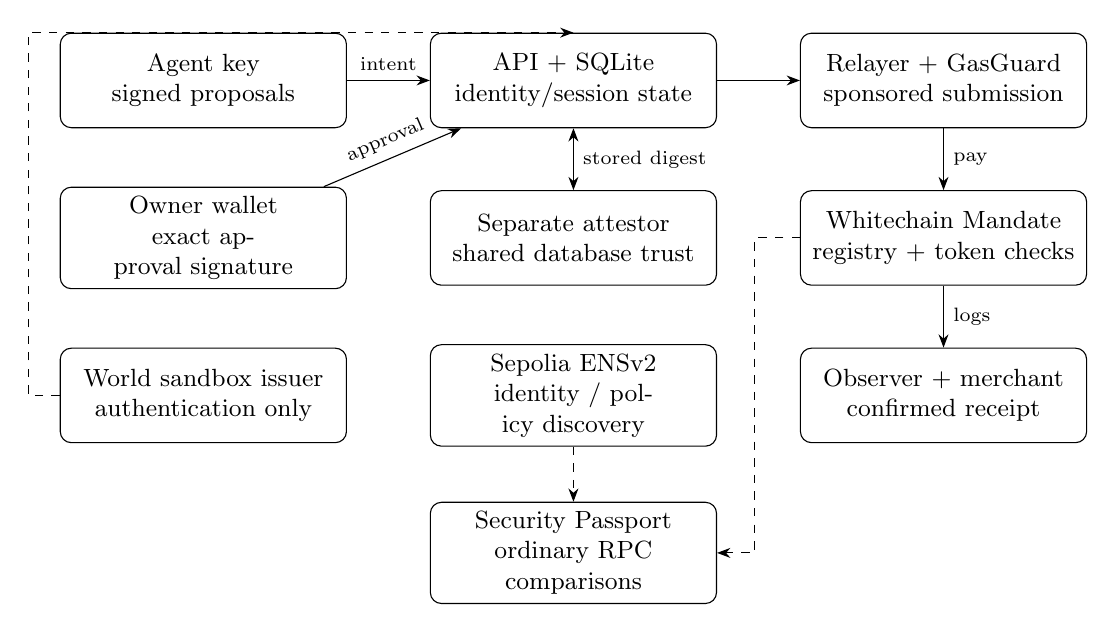
\begin{tikzpicture}[x=1cm,y=1cm,>=Stealth,box/.style={draw,rounded corners,align=center,font=\small,text width=34mm,minimum height=12mm}]
\node[box] (agent) at (0,0) {Agent key\\signed proposals};
\node[box] (api) at (4.7,0) {API + SQLite\\identity/session state};
\node[box] (relay) at (9.4,0) {Relayer + GasGuard\\sponsored submission};
\node[box] (owner) at (0,-2) {Owner wallet\\exact approval signature};
\node[box] (att) at (4.7,-2) {Separate attestor\\shared database trust};
\node[box] (chain) at (9.4,-2) {Whitechain Mandate\\registry + token checks};
\node[box] (world) at (0,-4) {World sandbox issuer\\authentication only};
\node[box] (ens) at (4.7,-4) {Sepolia ENSv2\\identity / policy discovery};
\node[box] (obs) at (9.4,-4) {Observer + merchant\\confirmed receipt};
\node[box] (passport) at (4.7,-6) {Security Passport\\ordinary RPC comparisons};
\draw[->] (agent)--node[above,font=\scriptsize]{intent}(api);
\draw[->] (api)--(relay);
\draw[->] (owner)--node[above,sloped,font=\scriptsize]{approval}(api);
\draw[<->] (api)--node[right,font=\scriptsize]{stored digest}(att);
\draw[->] (relay)--node[right,font=\scriptsize]{pay}(chain);
\draw[->] (chain)--node[right,font=\scriptsize]{logs}(obs);
\draw[->,dashed] (world.west) -- ++(-.4,0) |- (api.north);
\draw[->,dashed] (ens)--(passport);
\draw[->,dashed] (chain.west)--(7,-2)--(7,-6)--(passport.east);
\end{tikzpicture}
\caption{System and trust boundaries. Solid arrows carry signed requests, settlement calls or events; dashed arrows supply externally observed identity information. The owner, issuer, shared API/attestor database and chain are distinct trust assumptions. No ENS-to-Whitechain authority bridge exists.}\label{fig:architecture}
\end{figure}

\begin{figure}[htbp]\centering
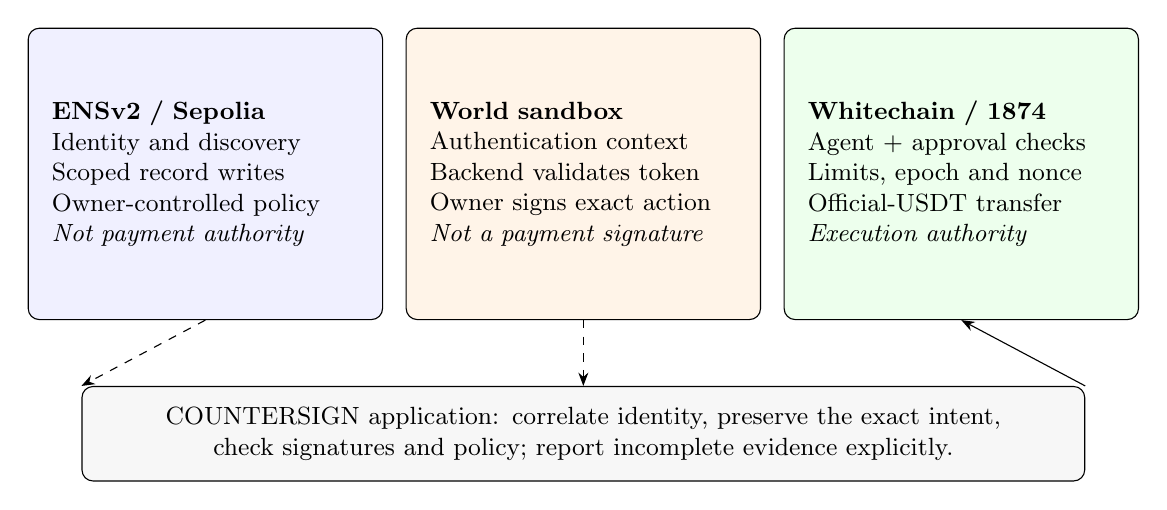
\begin{tikzpicture}[x=1cm,y=1cm,>=Stealth,
 panel/.style={draw,rounded corners,align=left,font=\small,text width=39mm,minimum height=37mm,inner sep=3mm}]
\node[panel,fill=blue!6] (ens) at (0,0) {\textbf{ENSv2 / Sepolia}\\Identity and discovery\\Scoped record writes\\Owner-controlled policy\\\textit{Not payment authority}};
\node[panel,fill=orange!9] (world) at (4.8,0) {\textbf{World sandbox}\\Authentication context\\Backend validates token\\Owner signs exact action\\\textit{Not a payment signature}};
\node[panel,fill=green!7] (pay) at (9.6,0) {\textbf{Whitechain / 1874}\\Agent + approval checks\\Limits, epoch and nonce\\Official-USDT transfer\\\textit{Execution authority}};
\node[draw,rounded corners,align=center,font=\small,text width=125mm,minimum height=12mm,fill=black!3] (app) at (4.8,-3.3) {COUNTERSIGN application: correlate identity, preserve the exact intent,\\check signatures and policy; report incomplete evidence explicitly.};
\draw[->,dashed] (ens.south)--(app.north west);
\draw[->,dashed] (world.south)--(app.north);
\draw[->] (app.north east)--(pay.south);
\end{tikzpicture}
\caption{Original authority map, derived from ENSv2 registry/resolver documentation~\cite{ensregistry,ensresolver}, World's application-owned action-approval boundary~\cite{worldstepup}, and the Whitechain testnet reference~\cite{whitechainnetwork}. Dashed edges carry identity observations; the solid edge submits a signed payment. No sponsor diagram or logo is reproduced, and no synchronous cross-chain authority is implied.}\label{fig:authority}
\end{figure}


\section{Protocol construction}
\subsection{Policy and funding}
A mandate identifier is the hash of the owner address and an owner-selected salt. The creator is the funding owner; there is no caller-supplied alternate treasury. A policy stores the agent and attestor addresses, maximum per-payment amount, period budget, human threshold, period origin and duration, mandate expiry, epoch and pause flag. Merchant permissions are a mapping under the mandate. The token and merchant registry are immutable constructor values.

The funding owner grants the Mandate a bounded token allowance. The contract cannot itself prohibit the owner from granting unlimited allowance; bounded setup is a client/deployment convention plus user action. The principal hard limit remains the contract policy, while a finite allowance adds an independent exposure bound. Multiple mandates belonging to the same owner have separate accounting but share that owner's token balance and allowance to the contract. No wallet-wide aggregate spending cap is provided.

A period is $k(t)=\lfloor(t-t_0)/\Delta\rfloor$, with start $t_0$ fixed at creation and duration $\Delta>0$. This is a tumbling period, not necessarily a calendar day or rolling 24-hour window. Historical period counters persist. Reducing a budget below spending already recorded does not undo that spending: the remaining balance saturates at zero, and subsequent payments fail until policy or period permits them. Refunds do not replenish counters.

\subsection{Typed messages and domain}
The domain is name ``Countersign'', version ``1'', the runtime chain identifier, and the particular Mandate address. The client fixes Whitechain Sepolia chain 1874; the contract uses the current chain identifier through the EIP-712 implementation. For intent $I$, approval $A$ and attestation $W$:
\begin{align*}
I={}&(m,q,p,v,a,o,r,n,e,d),\\
h_I={}&\operatorname{EIP712Hash}_{D}(I),\\
A={}&(h_I,m,q,p,a,e,d),\\
h_A={}&\operatorname{EIP712Hash}_{D}(A),\\
W={}&(h_A,s,t_{auth}).
\end{align*}
Here $m$ is mandate, $q$ merchant, $p$ payout, $v$ registry version, $a$ amount, $o$ order, $r$ request-resource hash, $n$ nonce, $e$ epoch, and $d$ deadline. $s$ is the backend's owner-subject hash. Complete field types and shared vectors are supplied in the artifact. The order and resource are transitively bound through $h_I$ even though not repeated in $A$.

Let $H$ denote Keccak-256 and $\operatorname{enc}$ Solidity ABI encoding of the statically typed fields. For a message of type $T$,
\begin{align}
 h_T(x)&=H\bigl(\operatorname{enc}(H(\operatorname{typeString}(T)),x)\bigr),\\
 \operatorname{digest}_D(x)&=H\bigl(\mathtt{0x1901}\Vert D\Vert h_T(x)\bigr).
\end{align}
Here $D$ is the EIP-712 domain separator, not the printable domain tuple. Every element in these messages is static; there is no ambiguous concatenation of variable-length strings. Appendix~\ref{app:types} gives field order and widths. Agent ECDSA recovery authenticates $h_I$ under the current policy agent. The owner verifies $h_A$ using ECDSA or ERC-1271; the attestor verifies the domain-separated digest of $W$ using ECDSA. Signer roles are selected from current policy, not from an untrusted supplied signer address.

Token identity is bound through immutable contract state and the verifying-contract domain, not an explicit field in $I$. There is no issuance-time field in $I$; freshness is represented by deadline, current epoch and the separate authentication time. The currently deployed protocol must not be described as implementing a larger hypothetical envelope. A resource hash commits to request bytes and cannot prove product truth, merchant legitimacy or fulfillment.

\subsection{Execution predicate and updates}
The payment function checks existence, pause, intent deadline, mandate expiry, epoch, nonce and paid-order uniqueness before checking merchant permission, current payout/version/active state, amount and period budget. It then verifies the agent signature. Amounts at or above the threshold require the owner and attestor checks. The owner signature uses the approval digest; the attestation must repeat that digest, contain a nonfuture authentication time no more than 300 seconds old, and recover the current attestor.

Write $U[m,n]$ for consumed nonces and $Q[H(\operatorname{enc}(m,q,o))]$ for paid orders. Ignoring revert labels, the main precondition is
\begin{align*}
 &P_m.owner\ne0\ \land\ \neg P_m.paused\ \land\ t\le d<t_{\infty},\qquad t<P_m.expiry,\\
 &e=P_m.epoch\ \land\ \neg U[m,n]\ \land\ \neg Q[H(\operatorname{enc}(m,q,o))],\\
 &\operatorname{allowed}(m,q)\ \land\ \operatorname{registry}(q)=(p,v,\mathrm{active}),\\
 &0<a\le P_m.perTxLimit\ \land\ spent_{m,k(t)}+a\le P_m.periodLimit,\\
 &\operatorname{agentValid}(h_I)\ \land\
 \bigl(a<P_m.humanThreshold\ \lor\ \operatorname{humanValid}(h_A,W)\bigr).
\end{align*}
Here $t$ is the block timestamp and $t_{\infty}=2^{64}$ is only the unsigned deadline encoding bound, not an implemented maximum approval lifetime. The human predicate requires the current owner's valid signature, $W.approvalDigest=h_A$, $0\le t-W.authTime\le300$, and the current attestor's valid signature. Transfer success additionally depends on token balance, allowance and token behavior. A preflight at time $t$ cannot guarantee these predicates at a later inclusion time.

Only after all checks does execution consume the nonce, increase the period counter and write the payment record. It then performs SafeERC20 transferFrom from the policy owner to the signed payout, and emits PaymentExecuted. ReentrancyGuard protects payment and refund entry points; a failed transfer reverts preceding state changes atomically. Because the per-payment limit is uint128, a successful amount can safely be stored in the uint128 payment field despite its wider signed input type.

A payment identifier hashes mandate, merchant and order. This is distinct from a nonce: a new nonce cannot pay the same order again, and the same nonce cannot pay a different order. Nonce usage remains consumed across epoch changes. Merchant allowlist changes, limit updates, agent rotation, attestor rotation and revoke each increment the epoch; pause changes do not. The contract does not bind the external caller to a designated relayer. Any caller possessing the complete valid authorization may submit it and pay gas. This is intentional permissionless execution, not permissionless authority to change its terms.

\section{Whitechain: enforceable spending and stablecoin settlement}
\subsection{Responsibility and implemented mechanism}
Whitechain is documented as an EVM-compatible OP Stack network~\cite{whitechain}. Its current Sepolia reference identifies chain 1874, WBT gas and the public testnet endpoints~\cite{whitechainnetwork}. These are documented configuration values, not measurements of COUNTERSIGN latency. The relayer accepts only the configured protected call, validates intent and policy, simulates execution, and reserves a bounded execution-gas budget through GasGuard. Signed transaction bytes, hash and account nonce are persisted before broadcast. On recovery, the same bytes may be resent. An ambiguous outcome is retained rather than silently replaced. This design assumes one dedicated signer and one active relayer process. It is not a horizontally scalable nonce coordinator.

The agent pays no execution gas on the demonstrated flow. The treasury pays for initial setup and token approval; the relayer funds WBT for subsequent execution. This is not universal gasless onboarding. Saved capability probes indicate permit and transferWithAuthorization interfaces are present, but a successful signed use of either remains unexecuted. A read-only signature or selector probe alone would not establish correct semantics. Full OP Stack fee accounting is distinct from limiting execution gas, and remains an operational limitation of the present guard.

An observer derives payment status from decoded contract logs after three blocks beyond inclusion. It checks block hashes, uses atomic persistence for projection and webhook outbox, and stops on detected reorganization. Three L2 blocks are an application confirmation policy, not a proof of Ethereum settlement finality. Whitechain distinguishes sequencer soft confirmation, safe inclusion and Ethereum-backed finalization~\cite{whitechainfinality}; this artifact does not benchmark those stages. A deep reorganization can require manual reconciliation of already delivered messages and resources.

The separate merchant application issues an HTTP 402 quote and releases its resource only after a checked receipt. The merchant SDK hides internal approval details while binding the request to the payment. Webhooks use authenticated payloads and retries; recipients still need event-id deduplication. Refunds are new transfers initiated by the original payout account, capped by the original payment and funded by that merchant. Neither the owner nor the server can forcibly reverse direct settlement. Duplicate partial refunds with remaining headroom can represent two valid refund transactions unless application-level idempotency prevents a second initiation.

\subsection{Financial enforcement and failure boundaries}
The configured official test USDT is immutable in the Mandate deployment. Its transfer originates from the mandate owner, who is also the funding account; an agent cannot choose another treasury merely because that treasury approved the contract. The MerchantRegistry binds payout and version, while the signed intent binds mandate, merchant, exact amount, order, resource hash, nonce, epoch and deadline. Per-transaction and period limits apply even when the owner has supplied a threshold approval. Consumed nonces and order records are updated in the same EVM transaction as the token transfer; a failed transfer rolls the state transition back. Reentrancy protection and safe token handling address separate token-call risks, not human identity.

Revocation and policy changes increment the epoch, so previously signed intents fail only after the changed state is included before execution. They do not cancel a transaction already executed, nor prohibit the current agent from signing a fresh-epoch intent. Spending counters survive policy changes and refunds. Bounded refunds require the recorded payout account to fund and authorize them; settlement is not a chargeback mechanism. These semantics are central Whitechain-side contributions of the implementation rather than features supplied by ENS records or World login.

\subsection{Evidence and next verification}
Local execution tests cover amount and payout mutation, per-transaction and period limits, duplicate orders, nonce reuse, domain confusion, signature checks, token-transfer failure, reentrancy and refunds. The invariant harness explores accounting and replay sequences. Repository records identify official-USDT transfers and selected mined reverts on Whitechain Sepolia; the manuscript does not infer the current deployed runtime from a local source file. The latest README additionally records a 0.50-USDT payment during a later video, separated from the earlier measured checkpoint. Independent receipt/runtime revalidation, durable production storage and a fresh integrated merchant journey remain distinct acceptance gates. Local mock-token gas observations do not measure Whitechain fee or confirmation distributions.

\begin{figure}[htbp]\centering
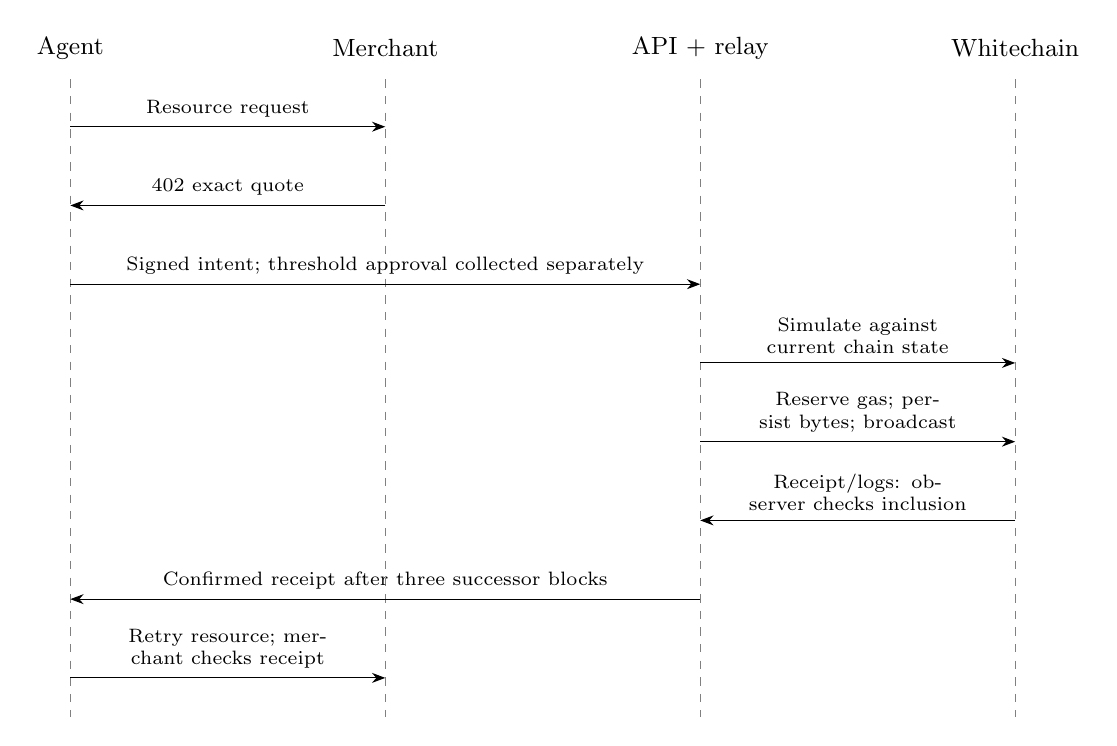
\begin{tikzpicture}[x=1cm,y=1cm,>=Stealth,font=\small]
\foreach \x/\name in {0/Agent,4/Merchant,8/API + relay,12/Whitechain}{\node at (\x,0){\name};\draw[dashed,gray] (\x,-.4)--(\x,-8.5);}
\draw[->] (0,-1)--node[above,font=\scriptsize]{Resource request}(4,-1);
\draw[->] (4,-2)--node[above,font=\scriptsize]{402 exact quote}(0,-2);
\draw[->] (0,-3)--node[above,font=\scriptsize]{Signed intent; threshold approval collected separately}(8,-3);
\draw[->] (8,-4)--node[above,font=\scriptsize,text width=36mm,align=center]{Simulate against current chain state}(12,-4);
\draw[->] (8,-5)--node[above,font=\scriptsize,text width=36mm,align=center]{Reserve gas; persist bytes; broadcast}(12,-5);
\draw[->] (12,-6)--node[above,font=\scriptsize,text width=36mm,align=center]{Receipt/logs: observer checks inclusion}(8,-6);
\draw[->] (8,-7)--node[above,font=\scriptsize]{Confirmed receipt after three successor blocks}(0,-7);
\draw[->] (0,-8)--node[above,font=\scriptsize,text width=36mm,align=center]{Retry resource; merchant checks receipt}(4,-8);
\end{tikzpicture}
\caption{Payment request and settlement sequence. A transaction hash alone does not release the resource. Observation is through RPC; the confirmation policy is not Ethereum finality. RPC errors and unknown outcomes do not become success.}\label{fig:payment}
\end{figure}

\section{World: fresh authentication and transaction-specific consent}
\subsection{Responsibility and implemented mechanism}
The API creates a persisted approval with a lifetime of at most 120 seconds, also bounded by the intent deadline. It generates random state, browser binding and a PKCE verifier. The nonce combines the approval digest with fresh randomness through SHA-256; it is not simply a deterministic hash of that digest. Starting a fresh authentication attempt does not create a new financial authorization.

The OIDC redirect uses authorization code flow, PKCE S256 and max\_age=0. The backend restricts discovery endpoints to the configured World issuer, validates a signed ID token using jose/JWKS, checks issuer, audience, nonce, subject, expiration, authentication time and any configured assurance class. Multiple audiences require a matching authorized-party claim in the approval state layer. The active authorization-code path does not unconditionally require an authentication-method claim. We therefore do not claim an assurance level beyond what configuration and the sandbox actually establish.

Successful authentication produces world\_ok, not permission to pay. The owner must still sign the exact EIP-712 PaymentApproval. A separate attestor process recomputes both stored digests, checks persisted state and freshness, atomically claims the approval, and signs once. The API rechecks current policy and simulates the full payment before relay. A crash after the attestor claim but before signature persistence is fail-closed but may require manual recovery. This trades availability for avoidance of uncontrolled repeated signing.

Cancellation is meaningful only before an externally usable authorization has escaped. A database denial cannot invalidate owner and attestor signatures already issued. Once they exist, the strongest invalidation is a Whitechain epoch change or pause effective before the payment executes. Nor does the backend's two-minute window shorten the already signed intent deadline on chain: a party holding signatures can submit directly while the intent and 300-second contract authentication bound remain valid. These distinct expiration boundaries must be shown accurately to users.

World's current OIDC guide specifies code flow with S256 PKCE and backend token validation~\cite{worldoidc}. Its step-up guide separately requires binding the attempt to the intended operation and account, checking freshness and any required assurance, and preserving application-owned approval~\cite{worldstepup}. Accordingly, COUNTERSIGN does not treat a successful authentication result as a payment signature. Assurance-class enforcement depends on the application's configured policy; a fresh sandbox login alone is not a claim of production Orb verification. The official testing guide explicitly separates sandbox credentials and local signed fixtures from production assurance~\cite{worldtesting}.

\subsection{Identity trust and explicit consent}
The separation between the issuer, application and owner wallet is essential. World authenticates the subject; the application binds that subject to the owner and checks the intended session; the wallet signs the displayed payment; the attestor asserts the stored authentication context; Whitechain verifies the supplied payment signatures and freshness bound. Neither a valid ID token alone nor the attestor alone can satisfy the threshold-payment predicate. Conversely, an owner signature does not demonstrate that the human understood the displayed terms, and a compromised identity database can mislead the attestor. Separate processes sharing a database are not independent identity witnesses.

The implemented cancellation route authenticates the initiating session and checks origin and current state. Concurrency tests exercise cancellation versus signature submission; failures must not be converted into settlement success. Once an externally usable owner/attestor authorization has been released, cancellation in application storage cannot erase it. Operators must distinguish refusal before signing from on-chain invalidation after an effective epoch change or pause.

\subsection{Evidence and next verification}
Locally signed JWT fixtures test invalid issuer/audience/nonce, wrong subject, stale authentication, expiry and denial; these are executable validation cases, not live issuer credentials. The preserved integration record separately documents a World sandbox sign-in followed by a 1.50-USDT payment, an expired approval without relay, and refusal of stale authentication. The sandbox's mocked identities establish protocol integration rather than production personhood. A subsequent complete browser ceremony against the release deployment, including exact-term display and a negative path, remains necessary. The evaluation does not combine these records into a claim that all historical demo runs succeeded.

\begin{figure}[htbp]\centering
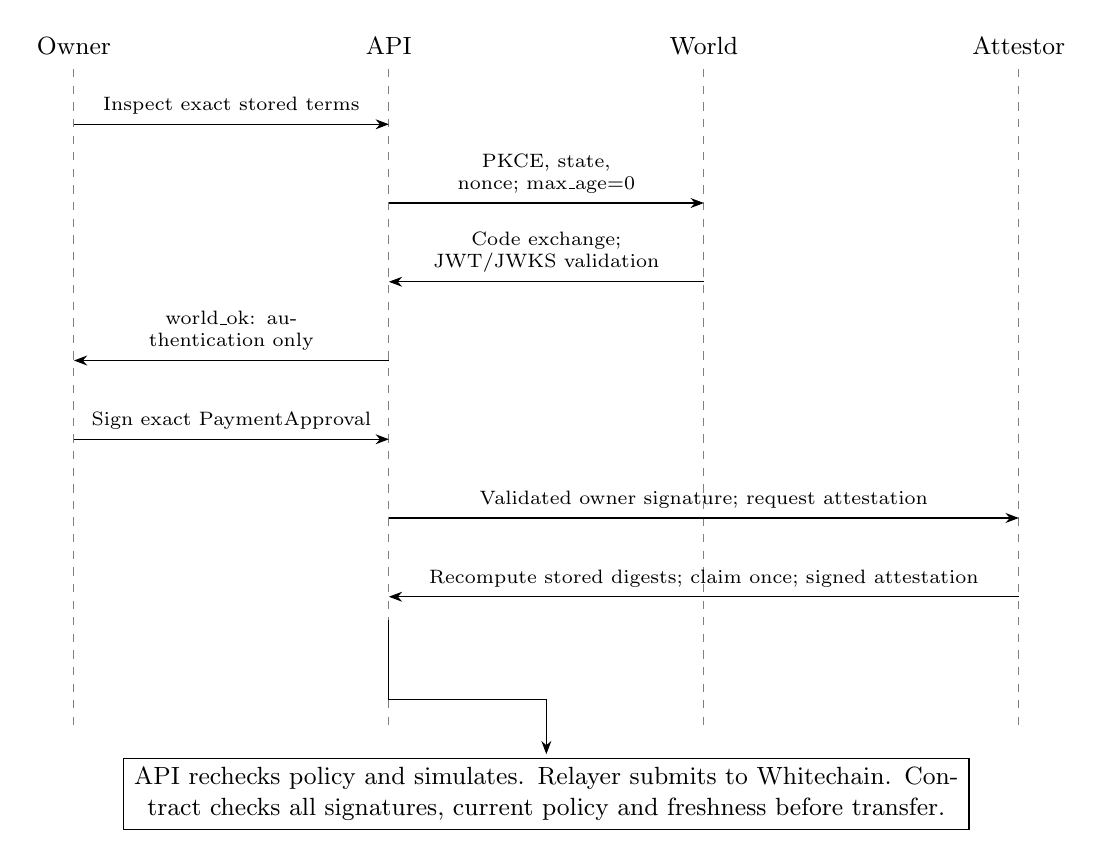
\begin{tikzpicture}[x=1cm,y=1cm,>=Stealth,font=\small]
\foreach \x/\name in {0/Owner,4/API,8/World,12/Attestor}{\node at (\x,0){\name};\draw[dashed,gray] (\x,-.3)--(\x,-8.7);}
\draw[->] (0,-1)--node[above,font=\scriptsize,text width=36mm,align=center]{Inspect exact stored terms}(4,-1);
\draw[->] (4,-2)--node[above,font=\scriptsize,text width=36mm,align=center]{PKCE, state, nonce; max\_age=0}(8,-2);
\draw[->] (8,-3)--node[above,font=\scriptsize,text width=36mm,align=center]{Code exchange; JWT/JWKS validation}(4,-3);
\draw[->] (4,-4)--node[above,font=\scriptsize,text width=36mm,align=center]{world\_ok: authentication only}(0,-4);
\draw[->] (0,-5)--node[above,font=\scriptsize,text width=36mm,align=center]{Sign exact PaymentApproval}(4,-5);
\draw[->] (4,-6)--node[above,font=\scriptsize]{Validated owner signature; request attestation}(12,-6);
\draw[->] (12,-7)--node[above,font=\scriptsize]{Recompute stored digests; claim once; signed attestation}(4,-7);
\node[draw,align=center,text width=105mm,font=\small] at (6,-9.5) {API rechecks policy and simulates. Relayer submits to Whitechain. Contract checks all signatures, current policy and freshness before transfer.};
\draw[->] (4,-7.3)--(4,-8.3)--(6,-8.3)--(6,-9);
\end{tikzpicture}
\caption{Threshold-payment authorization. World authenticates; the owner signs the financial action. Denial, expiry and subject mismatch stop the backend path. A later database cancellation cannot invalidate signatures already released.}\label{fig:approval}
\end{figure}


\section{ENSv2: discoverable identity and delegated record authority}
\subsection{Responsibility and implemented mechanism}
The prototype records an agent name under countersign.eth on Sepolia, with a dedicated UserRegistry and PermissionedResolver. It publishes the Whitechain mandate reference, limits, attestor and epoch. Agent-scoped setter roles cover endpoint/context records; policy keys remain owner-controlled. ENSv2's resource-specific access control is suited to this separation~\cite{ens,ensregistry,ensresolver}. The operational keys follow draft ENSIP-26, whereas the policy keys are application-specific~\cite{ensip26}. The current proof records role grants and name/address resolution. A live negative test showing the agent cannot alter an owner-only record, and a complete revocation lifecycle demonstration, should accompany a stronger release.

\subsection{Permission scope and cross-chain limits}
The resolver permission resource deserves a precise interpretation. A text-key setter role applies to that key across the resolver, not to one ENS name by itself. A dedicated resolver for an agent is therefore part of the isolation design; assigning multiple agents to one resolver changes the authority boundary. Namespace ownership, resolver administration and text-key setters must not be presented as interchangeable privileges.

The later release adds a browser-callable Security Passport that reads both chains at identified blocks, rechecks block hashes, compares available fields and hashes a canonical evidence object. Its policy commitment is computed from the read inputs; it is not a new value already committed by the deployed contract. Missing merchant-set aggregation and unenumerated ownership or administration checks prevent a whole-passport VERIFIED claim. A zero ENS namehash in a mandate also does not establish an owner-selected name binding. The evidence hash detects changed bytes relative to a known hash, not a dishonest RPC or an authoritative signature. A later integration checkpoint adds a locally tested historical payment verifier and optional persistent ENS relay gate. The verifier checks receipt/calldata consistency, official-token transfers, signatures and reconstructible historical policy against independent deployment anchors. It returns UNVERIFIED for earlier same-block policy events requiring traces, missing archive state or unsupported historical ERC-1271 validation. Its ENS and payment blocks are separately identified rather than assumed simultaneous. The monitor persists snapshots and a bounded configured-contract log journal, resumes backfill and quarantines reorgs. It intentionally refuses currently partial passports; no new live verifier or monitor result is claimed. These additions extend the implementation, not the historical gas experiment.

\begin{figure}[htbp]\centering
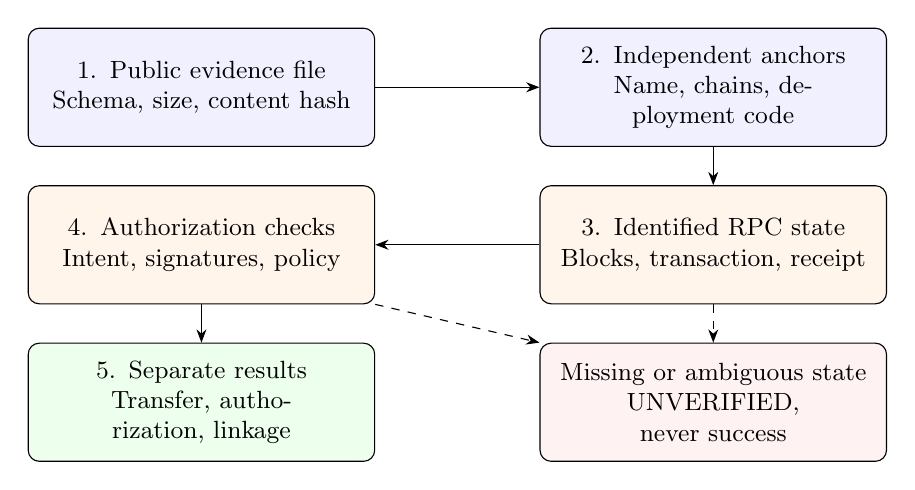
\begin{tikzpicture}[x=1cm,y=1cm,>=Stealth,
 box/.style={draw,rounded corners,align=center,font=\small,text width=40mm,minimum height=15mm,inner sep=2mm}]
\node[box,fill=blue!6] (file) at (0,0) {1. Public evidence file\\Schema, size, content hash};
\node[box,fill=blue!6] (anchor) at (6.5,0) {2. Independent anchors\\Name, chains, deployment code};
\node[box,fill=orange!8] (rpc) at (6.5,-2) {3. Identified RPC state\\Blocks, transaction, receipt};
\node[box,fill=orange!8] (auth) at (0,-2) {4. Authorization checks\\Intent, signatures, policy};
\node[box,fill=green!7] (scope) at (0,-4) {5. Separate results\\Transfer, authorization, linkage};
\node[box,fill=red!5] (limit) at (6.5,-4) {Missing or ambiguous state\\UNVERIFIED, never success};
\draw[->] (file)--(anchor);
\draw[->] (anchor)--(rpc);
\draw[->] (rpc)--(auth);
\draw[->] (auth)--(scope);
\draw[->,dashed] (rpc)--(limit);
\draw[->,dashed] (auth.south east)--(limit.north west);
\end{tikzpicture}
\caption{Original diagram of the later locally tested payment verifier. File hashes prove integrity only relative to a trusted hash. Ordinary RPC reads do not supply consensus proofs. Earlier same-block policy mutations, unsupported historical smart-wallet validation or unavailable archive data prevent complete verification. No new live-chain result is implied.}\label{fig:verification}
\end{figure}


ENS is outside the synchronous Whitechain enforcement boundary. Off-chain reads can be cached, unavailable or stale; a resolver edit does not mutate Mandate state. A drift view compares visible policy records with current chain reads, but one field, the merchant-set hash, lacks a direct equivalent in the deployed mapping. It must remain missing rather than be shown as matched. The namehash stored by the payment policy is not a bridge or oracle.

Immediate payment invalidation requires a Whitechain policy update subject to ordering and inclusion. Namespace permission changes constrain future ENS writes, not existing Whitechain signatures. The ENS management command does not execute a Whitechain revoke. Even a future two-chain command could not make these changes atomic. If the ENS transaction succeeds but the Whitechain transaction fails, the operator must report partial completion and retry the correct chain action without implying that payments are disabled.

\subsection{Evidence and next verification}
Recorded ENS evidence covers registration, resolver configuration, text records and scoped grants. It does not by itself demonstrate that every forbidden write or permission escalation reverts under the deployed administration. A harness compiles against the deployed interfaces, while RPC failures prevented execution at the saved checkpoint. Local passport/monitor tests use fixture RPCs and must remain a separate evidence category. Next verification should execute owner recovery, forbidden policy editing, cross-agent isolation and revocation against the actual role model, preserving the independent Whitechain policy throughout. ENS is therefore evaluated as an identity and record-permission integration, not a substitute for settlement or human authentication.

\begin{figure}[htbp]\centering
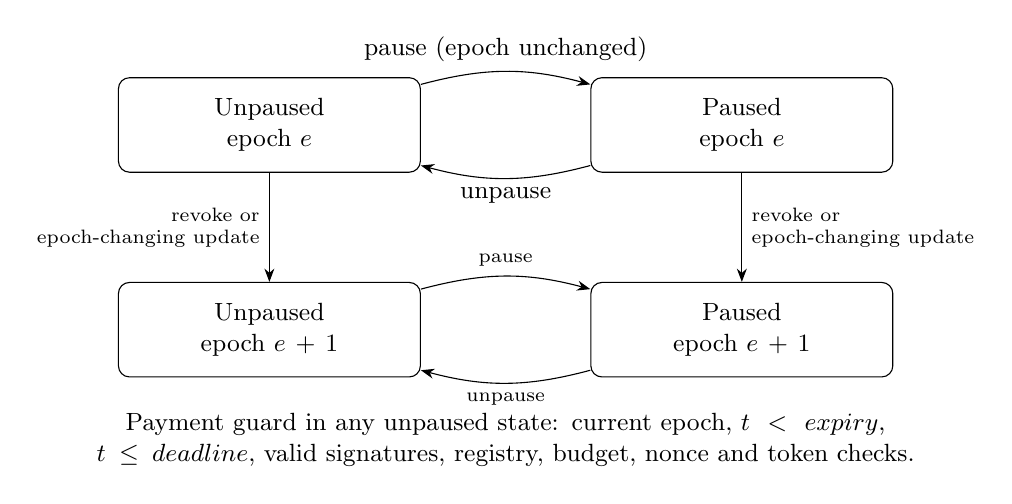
\begin{tikzpicture}[x=1cm,y=1cm,>=Stealth,box/.style={draw,rounded corners,align=center,font=\small,text width=36mm,minimum height=12mm}]
\node[box] (a) at (0,0) {Unpaused\\epoch $e$};
\node[box] (p) at (6,0) {Paused\\epoch $e$};
\node[box] (b) at (0,-2.6) {Unpaused\\epoch $e+1$};
\node[box] (q) at (6,-2.6) {Paused\\epoch $e+1$};
\draw[->] (a) to[bend left=15] node[above,font=\small]{pause (epoch unchanged)} (p);
\draw[->] (p) to[bend left=15] node[below,font=\small]{unpause} (a);
\draw[->] (a)--node[left,font=\scriptsize,align=right]{revoke or\\epoch-changing update} (b);
\draw[->] (p)--node[right,font=\scriptsize,align=left]{revoke or\\epoch-changing update} (q);
\draw[->] (b) to[bend left=15] node[above,font=\scriptsize]{pause} (q);
\draw[->] (q) to[bend left=15] node[below,font=\scriptsize]{unpause} (b);
\node[align=center,font=\small,text width=115mm] at (3,-4) {Payment guard in any unpaused state: current epoch, $t<expiry$, $t\le deadline$, valid signatures, registry, budget, nonce and token checks.};
\end{tikzpicture}
\caption{Administrative transitions preserve the pause flag when changing epoch. Revoke invalidates old-epoch signatures but leaves fresh-epoch payments possible. Pause/unpause alone can revive an unexpired unused signature. Expiry is an execution guard, not a stored terminal state.}\label{fig:state}
\end{figure}

\begin{figure}[htbp]\centering
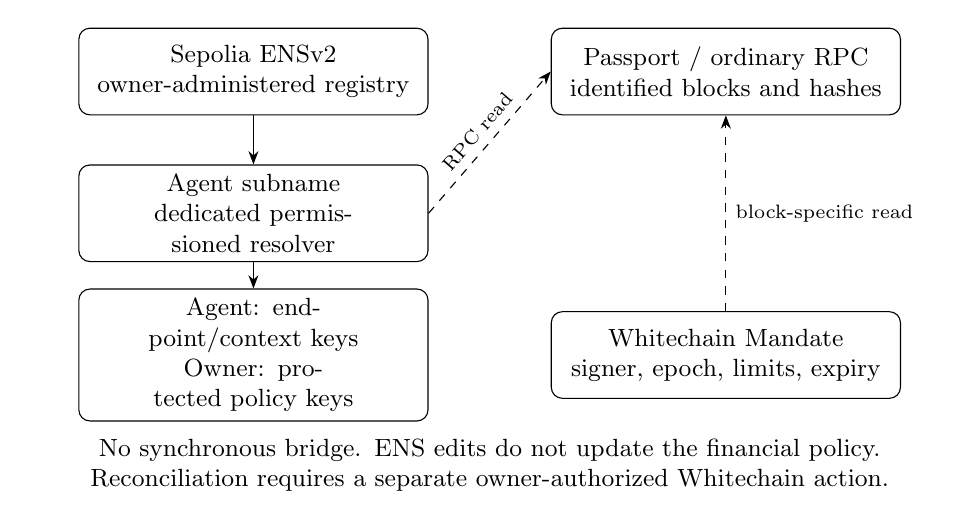
\begin{tikzpicture}[x=1cm,y=1cm,>=Stealth,box/.style={draw,rounded corners,align=center,font=\small,text width=42mm,minimum height=11mm}]
\node[box] (root) at (0,0) {Sepolia ENSv2\\owner-administered registry};
\node[box] (res) at (0,-1.8) {Agent subname\\dedicated permissioned resolver};
\node[box] (read) at (6,0) {Passport / ordinary RPC\\identified blocks and hashes};
\node[box] (pay) at (6,-3.6) {Whitechain Mandate\\signer, epoch, limits, expiry};
\node[box] (roles) at (0,-3.6) {Agent: endpoint/context keys\\Owner: protected policy keys};
\draw[->] (root)--(res);
\draw[->] (res)--(roles);
\draw[->,dashed] (res.east)--node[above,sloped,font=\scriptsize]{RPC read}(read.west);
\draw[->,dashed] (pay)--node[right,font=\scriptsize]{block-specific read}(read);
\node[font=\small,align=center,text width=115mm] at (3,-5) {No synchronous bridge. ENS edits do not update the financial policy.\\Reconciliation requires a separate owner-authorized Whitechain action.};
\end{tikzpicture}
\caption{ENS permissions and cross-chain trust. Setter scope is a text key across a resolver, so dedicated resolvers are required for the claimed agent isolation. Ordinary RPC observations can detect disagreement but are not cross-chain proofs. Recorded grants exist; permission-negative/revocation fork execution is blocked.}\label{fig:ens}
\end{figure}

\section{Security properties and argument}
For a successful payment transition $S\rightarrow S'$, let $P_m$ be the policy evaluated in $S$. The intended integrity property is that transfer token equals the immutable token, source equals $P_m.owner$, and recipient/amount equal the validated intent. Unforgeability and collision resistance support the inference from a valid signature to signed field agreement; correct implementation of encoding and signature validation remains an assumption tested by fixed vectors and adversarial cases.

Budget safety is a transition property: $spent_{m,k}+a\leq limit_m$ before each accepted execution, and $spent'_{m,k}=spent_{m,k}+a$. It is not the assertion that historical spending can never exceed a subsequently lowered limit. Nonce uniqueness requires that acceptance implies $used'_{m,n}=true$ and all later executions using $(m,n)$ fail. Paid-order uniqueness independently covers $(m,q,o)$.

Revocation safety must be expressed as epoch invalidation: after epoch $e$ changes, an intent carrying $e$ cannot execute. The function named revoke does not permanently disable the mandate; an agent can sign a fresh intent with the new epoch. Pause blocks new payments while true, but unpausing can revive an unexpired previously signed intent if no epoch-changing action occurred. Administrative semantics therefore matter as much as the existence of a revoke button.

For a high-threshold payment, owner and attestor signatures must agree on $h_A$, which includes $h_I$. An authorization for order A therefore does not authorize order B under unchanged signatures. This is a cryptographic agreement property, not proof of informed human consent. Authentication-subject correctness is asserted by the attestor and backend, not established cryptographically by Whitechain itself.

Settlement consistency requires that a returned settled status be derived from a matching observed event under the configured confirmation policy. It does not require every submitted transaction to settle: expiry, balance changes, nonce races or ordering may legitimately cause reverts. Availability and failure recovery are evaluated separately. These are specification-level arguments; no mechanized theorem or independent audit is claimed.

\begin{table}[htbp]\centering\small
\begin{tabular}{p{.22\linewidth}p{.40\linewidth}p{.28\linewidth}}\toprule
Property & Scope / counterexample boundary & Executed local evidence\\\midrule
Payment integrity & Signed fields and immutable token; not fulfillment & T02, T03, T22; digest vectors\\
Budget safety & Accepted transition respects current period cap; lowered cap may be below historical spend & T06--T09, T30 invariant\\
Nonce/order uniqueness & Per-mandate nonce and paid-order maps; epoch does not reset usage & T10, T11\\
Approval binding & Exact intent hash under current owner/attestor; no proof of understanding & T12--T15; different-order regression\\
Revocation & Old epoch fails; fresh-epoch intent can succeed & T16, T17; fresh-epoch regression\\
Pause & Reject while paused; does not destroy unused signatures & T20; unpause-revival regression\\
Settlement projection & Matching canonical log under confirmation policy; deep reorg requires recovery & Observer range/runner fixtures\\\bottomrule
\end{tabular}
\caption{Security specifications and test mappings. T-labels refer to named contract tests; finite tests and invariant fuzzing are not mathematical proofs.}\label{tab:properties}
\end{table}

\begin{table}[ht]\centering\small
\begin{tabular}{p{.26\linewidth}p{.32\linewidth}p{.31\linewidth}}\toprule
Attacker action & Enforced boundary & Evidence / residual risk\\\midrule
Change amount or payout & Agent/owner digest and registry & Local tests; recorded mined reverts\\
Reuse nonce/order & Contract replay maps & Local tests; order binding case\\
Old epoch after revoke & Current policy equality & Local tests; recorded API rejection\\
Forge identity state & Backend/attestor trust & Not solved by on-chain JWT verification\\
Spend after ENS role edit & Whitechain policy unchanged & Not an immediate payment kill switch\\
Replay webhook & Recipient event deduplication & Local tests; transport alone insufficient\\
Delay broadcast/reorg & Deadline, observer hash checks & Availability/manual recovery remain\\
Owner key compromise & Outside owner trust assumption & Wallet-wide protection not provided\\\bottomrule
\end{tabular}
\caption{Attack/defense matrix. Local tests, recorded live outcomes and non-guarantees are deliberately distinguished. Full scenario mapping is in the security artifact.}
\end{table}

\section{Implementation and reproducibility}
The implementation uses Solidity 0.8.30 targeting Prague, optimizer 200 and via-IR, with OpenZeppelin Contracts 5.4.0. Shared viem typed data and fixed vectors exercise digest parity with Solidity. The service uses Node.js, SQLite persistence, jose validation and WebSocket invalidation notifications. Browser events trigger fresh authoritative reads; a socket event cannot itself authorize or settle a payment. The ENS package pins viem 2.35.0; exact resolved dependencies are in lockfiles, not inferred from manifest ranges.

The artifact separates source, local raw results and historical public-chain evidence. Scripts record commands and environments; sources are keyed to the repository revision and working-tree state. A reader should first reproduce unit/invariant tests, then inspect the benchmark measurement scope, then reproduce testnet steps with their own credentials and sponsor tokens. Mock ERC20 contracts are restricted to local tests. No issuer credentials, keystore secrets or private signing material should enter the research bundle.

\begin{table}[htbp]\centering\small
\begin{tabular}{p{.23\linewidth}p{.34\linewidth}p{.33\linewidth}}\toprule
Component & Implementation / trust & Reproduction pointer\\\midrule
Settlement & Solidity 0.8.30, Prague, via-IR, optimizer 200; OZ 5.4.0 & \code{contracts/src/}; local mock-token test suite\\
Typed signing & Three messages; owner ERC-1271 support & \code{packages/shared/}; fixed vectors\\
Identity service & Node 24.10.0 checkpoint, SQLite, jose & \code{apps/api/}; signed local JWT fixtures\\
Attestor & Separate signer process, shared database trust & \code{apps/attestor/}; not independent enrollment proof\\
ENS passport & Block-specific RPC reads, partial comparisons & \code{packages/ens/}; no trustless cross-chain bridge\\\bottomrule
\end{tabular}
\caption{Implementation configuration and trust-relevant scope. Lockfiles, source hashes and raw logs identify the exact artifact; no clean-machine deployment claim is made.}\label{tab:implementation}
\end{table}

\section{Evaluation and measured findings}
The recorded research-checkpoint rerun passed 99 Node tests, 131 Solidity tests (including four local benchmark cases and inherited repetitions), three shared digest-vector tests, signed local JWT fixtures, and frontend lint/type checks. Counts include inherited Solidity tests repeated in derived suites; they are not counts of distinct security properties. The invariant configuration uses 256 runs and depth 64. The final checkpoint includes new cases for order-specific owner approval, fresh-intent validity after epoch revocation, and revival after pause/unpause, plus backend cancellation and attestation-ordering regressions. A passing local JWT fixture is not a real World verification.

A subsequent release checkpoint records 108 Node tests and the same 131 Solidity test executions, with digest, JWT-fixture, lint, type and format checks passing. It adds direct-RPC passport and authenticated end-user cancellation coverage. Its logs reside in \code{docs/proof/release/}; these are a separate checkpoint and do not replace the research measurements in \code{research/results/}. Final release reruns belong in a new evidence directory and must be consulted for the actual released revision. This manuscript does not infer live ENS permission transitions, browser acceptance or complete demo runs from either local suite. A fresh final-checkout rerun subsequently passed 109 Node tests, 131 Solidity test executions, three digest-vector tests, signed JWT fixtures, lint, type and formatting checks, recorded in \code{docs/evidence/final/final-checks/}. ENS fork tests compiled but could not execute because RPC DNS resolution failed; browser and production-build attempts were blocked by environment permissions. These are blocked gates, not passing integration tests.

\begin{table}[htbp]\centering\small
\begin{tabular}{p{.30\linewidth}p{.20\linewidth}p{.40\linewidth}}\toprule
Evidence item & Outcome & Interpretation\\\midrule
Earlier Node suite & 109 passed & Historical release checkpoint\\
Later Node integration & 154 passed & Monitor, verifier and wallet fixtures; separate checkpoint\\
Solidity suite & 131 executions & Includes inherited repetitions and four benchmark cases\\
Shared digest vectors & 3 passed & Local viem/Solidity encoding agreement\\
ENS deployed-state fork & Compiled only & Execution blocked by RPC DNS failure\\
World JWT fixtures & Passed locally & Locally signed tokens, not issuer interaction\\
World sandbox payment & Recorded & Actual sandbox issuer; mocked identity assurance\\
Six-step live demos & 5/6 each & Two incomplete runs, not full end-to-end success\\
Browser / fresh chain reads & Blocked & No fresh independent acceptance in this pass\\\bottomrule
\end{tabular}
\caption{Evidence classes must not be combined into a single completion or success percentage. The later integration logs are in \code{docs/evidence/integration/checks-release/}; neither checkpoint changes the historical gas data.}\label{tab:evidence}
\end{table}

\subsection{Balanced integration evidence}
The three integrations are compared on the same axes in Table~\ref{tab:three-integrations}. Equal analytical attention does not imply equal experimental coverage. The payment layer has recorded settlement receipts, the authentication layer has a recorded sandbox ceremony, and deployed-state negative ENS permission tests remain incomplete. These are intentionally different findings.

\begin{table}[htbp]\centering\small
\begin{tabular}{p{.16\linewidth}p{.27\linewidth}p{.25\linewidth}p{.22\linewidth}}\toprule
Integration & Enforced / validated boundary & Recorded evidence & Still not established\\\midrule
Whitechain & Exact protected transfer; limits, merchant/version, replay and epoch & Local contract executions; official-USDT txs and selected reverts & Current runtime revalidation; matched network performance; complete current journey\\
World & Backend authentication validation; owner/session binding; exact owner approval remains separate & Signed local JWT fixtures; sandbox login-to-payment; expiry/stale refusal & Production personhood; trusted display; complete release browser ceremony\\
ENSv2 & Registry/resolver identity; scoped record administration; observational policy comparison & Registration, scoped grants, records; local verifier tests & Executed deployed-state negative/revocation suite; synchronous cross-chain enforcement\\\bottomrule
\end{tabular}
\caption{Parallel evaluation of Whitechain, World and ENSv2. Evidence is classified by observation type rather than sponsor importance.}\label{tab:three-integrations}
\end{table}

A current presentation-preparation rerun executed 157 Node tests with no failures or skips; its log is \code{presentation/evidence/node-tests.txt}. It does not replace the earlier 109/154-test checkpoints, the 131-execution Solidity record or the gas dataset. The current README at revision \code{5688b18} reports a later recorded video and payment and Cloudflare/Render hosting. This pass could not independently retrieve those public endpoints. Consequently those additions are attributed to repository records, not reported as fresh network observations by the manuscript authoring process.

\subsection{Exploratory local gas experiment}
Four instrumented local tests compare direct ERC20 transfer, delegated allowance transferFrom, automatic COUNTERSIGN pay, and a human-signature fixture pay. The measured gasleft differences are respectively 58,236, 59,636, 240,671 and 258,628 gas, with one sample per configuration. This is a measured execution-region microbenchmark, not transaction receipt gas. Setup, intrinsic transaction gas, off-chain signing and identity interaction are excluded. Storage/access warmness is not normalized, and setup/access paths differ despite equal transfer amounts. The allowance baseline is a minimal primitive, not a feature-equivalent competitor. These limitations preclude claiming a robust overhead percentage, speedup, throughput or statistically established latency.

\begin{table}[ht]\centering
\begin{tabular}{lr}\toprule Local instrumented region & Gas, single sample\\\midrule
Direct ERC20 transfer & 58,236\\
Delegated ERC20 allowance transfer & 59,636\\
COUNTERSIGN automatic & 240,671\\
COUNTERSIGN human-signature fixture & 258,628\\\bottomrule\end{tabular}
\caption{Exploratory local mock-token measurements. Raw data and analysis script accompany the artifact. Do not interpret these as public-testnet transaction fees.}\end{table}

\begin{figure}[htbp]\centering
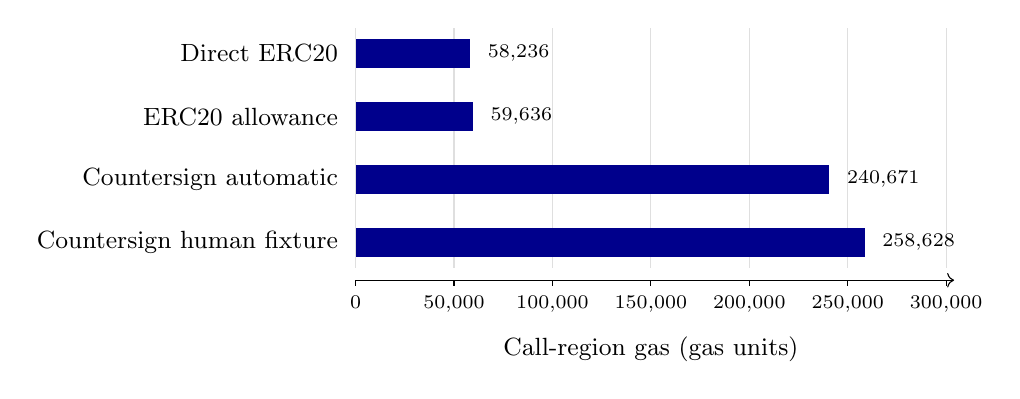
\begin{tikzpicture}[x=1cm,y=.8cm,font=\small]
\draw[->] (0,-3.6)--(7.6,-3.6);\node at (3.75,-4.7) {Call-region gas (gas units)};
\draw[gray!25] (0.0000,-3.4)--(0.0000,.4);
\draw (0.0000,-3.6)--(0.0000,-3.7) node[below,font=\scriptsize] {0};
\draw[gray!25] (1.2500,-3.4)--(1.2500,.4);
\draw (1.2500,-3.6)--(1.2500,-3.7) node[below,font=\scriptsize] {50,000};
\draw[gray!25] (2.5000,-3.4)--(2.5000,.4);
\draw (2.5000,-3.6)--(2.5000,-3.7) node[below,font=\scriptsize] {100,000};
\draw[gray!25] (3.7500,-3.4)--(3.7500,.4);
\draw (3.7500,-3.6)--(3.7500,-3.7) node[below,font=\scriptsize] {150,000};
\draw[gray!25] (5.0000,-3.4)--(5.0000,.4);
\draw (5.0000,-3.6)--(5.0000,-3.7) node[below,font=\scriptsize] {200,000};
\draw[gray!25] (6.2500,-3.4)--(6.2500,.4);
\draw (6.2500,-3.6)--(6.2500,-3.7) node[below,font=\scriptsize] {250,000};
\draw[gray!25] (7.5000,-3.4)--(7.5000,.4);
\draw (7.5000,-3.6)--(7.5000,-3.7) node[below,font=\scriptsize] {300,000};
\node[anchor=east,font=\small] at (-.1,0) {Direct ERC20};
\fill[blue!55!black] (0,-0.23) rectangle (1.4559,0.23);
\node[anchor=west,font=\scriptsize] at (1.5559,0) {58,236};
\node[anchor=east,font=\small] at (-.1,-1) {ERC20 allowance};
\fill[blue!55!black] (0,-1.23) rectangle (1.4909,-0.77);
\node[anchor=west,font=\scriptsize] at (1.5909,-1) {59,636};
\node[anchor=east,font=\small] at (-.1,-2) {Countersign automatic};
\fill[blue!55!black] (0,-2.23) rectangle (6.0168,-1.77);
\node[anchor=west,font=\scriptsize] at (6.1168,-2) {240,671};
\node[anchor=east,font=\small] at (-.1,-3) {Countersign human fixture};
\fill[blue!55!black] (0,-3.23) rectangle (6.4657,-2.77);
\node[anchor=west,font=\scriptsize] at (6.5657,-3) {258,628};
\end{tikzpicture}
\caption{Local mock-token call-region gas, $n=1$ per configuration. Generated from the recorded gas CSV and benchmark trace. Setup, intrinsic gas and off-chain authentication are excluded; access warmness is not normalized. No error bars or inferential statistics are warranted. Not public-testnet fees or latency.}\label{fig:gas}
\end{figure}

\subsection{Historical public-testnet evidence}
Recorded deployment evidence names MerchantRegistry at
\href{https://explorer.testnet.whitechain.io/address/0x2686f693A2C959568e650e0A5563E6244f2329E2}{0x2686...29E2} and Mandate at
\href{https://explorer.testnet.whitechain.io/address/0x923298375911A173da34C715da2718c0c9889EbA}{0x9232...9EbA} on chain 1874. A verification log reports both sources verified after an explorer outage. The first official-USDT payment is linked in Appendix~\ref{app:evidence}. A later protected payment followed a real World sandbox sign-in, an owner signature and attestor signing. The provider's sandbox uses mocked identities: this proves integration with that issuer, not production personhood assurance.

The live approval command retained the label order-40 but used 1.50 USDT against a 1.00-USDT threshold. Reporting it as a 40-USDT settlement would be incorrect. Expired and stale-authentication attempts were recorded as refused without extra relay transactions. The acceptance record has 14 of 16 cases marked pass; registry-change-after-approval and real browser-wallet dashboard interactions were still open at its checkpoint. Two six-step demo runs each achieved five steps before waiting on World. A later standalone success does not turn those earlier runs into two complete six-step executions.

Mined revert evidence includes amount-signature mismatch, payout/version mismatch, a per-transaction limit violation, pause and excessive refund. The over-budget case is specifically OverPerTx and must not be cited as a live OverPeriod demonstration. Revoke replay evidence records API StaleEpoch rejection rather than a mined revert. Testnet observations are evidence of the demonstrated cases, not a population success-rate estimate. Current public service uptime and independent transaction revalidation are separate checks from reading saved records.

\section{Limitations and research validity}
The system has not been independently audited, and this draft is not a formal proof. Full backend compromise can falsify identity persistence; owner-key compromise can authorize arbitrary exact payments within or after changed policy. Human understanding is not established by a signature, and the frontend/wallet rendering path requires further adversarial evaluation. Threshold splitting remains allowed within period limits: several small payments may avoid step-up. This behavior may be policy-correct yet undesirable for some organizations.

The token contract is trusted to implement expected transfer semantics. The prototype is not designed for fee-on-transfer, rebasing or adversarial upgrade behavior without further accounting checks. A limited allowance can be exhausted by another authorized mandate. An RPC can deny service or provide inconsistent observations; current detection is not a trustless light-client verification protocol. Reorganizations can invalidate previously delivered resources, and automatic compensation is not provided.

Cross-chain ENS consistency is observational, not atomic. Sandbox identity results do not establish production assurance. The earlier demo used a laptop-dependent tunnel. The later README reports a Cloudflare frontend and a Render API/attestor deployment; that record also discloses idle sleep, ephemeral storage and co-location of the two signing-related processes. This pass did not independently verify uptime or recovery. Hosting configuration is therefore not evidence of durable production operation. Historical documents contain superseded checkpoints; the artifact audit records provenance rather than treating every past statement as current. Git commit dates provide development evidence but cannot alone establish originality or hackathon eligibility of imported code.

The gas experiment has no replication or equivalence controls adequate for comparative scientific claims. There are no measured distributions for end-to-end latency, human effort, failure recovery duration or throughput. There is no user study. The next research phase should implement a feature-matched delegated/smart-account baseline, repeat randomized equivalent workloads, archive receipts and clocks, predefine failure classification, and analyze uncertainty without treating repeated deterministic EVM executions as independent human observations.

\section{Discussion and conclusion}
Whitechain, World and ENSv2 contribute different parts of one authorization path: financial enforcement, fresh human authentication context, and inspectable agent identity. None provides the complete path on its own. A useful authorization system must preserve its distinctions at failure boundaries. Authentication differs from permission; a proposal differs from signed consent; broadcast differs from inclusion; inclusion differs from application confirmation; and identity metadata differs from settlement authority. COUNTERSIGN makes these boundaries explicit in an implemented prototype and a testable artifact, with historical integration evidence and current verification gaps. Its strongest present evidence concerns implemented transaction/policy checks and recorded testnet integration, not novelty or production readiness.

The appropriate publication trajectory is an author-reviewed technical report followed by a controlled comparative evaluation. Related work already offers transaction-bound approval and formal agent-payment analysis. A defensible extension would compare concrete enforcement and failure-recovery behavior under equivalent attack and workload models, including counterexamples and operational costs. The current artifact supplies a starting point and exposes limits that a promotional description could hide.

\begin{table}[htbp]\centering\small
\begin{tabular}{p{.28\linewidth}p{.32\linewidth}p{.30\linewidth}}\toprule
Limitation & Consequence & Evidence needed next\\\midrule
Untrusted display / owner compromise & Valid signature need not imply informed consent & Adversarial rendering study\\
Separate chains / ordinary RPC & Drift reads do not revoke financial authority & Fork/live roles and robust historical reads\\
Shared identity database & Attestor is not an independent identity oracle & Stronger isolation and compromise evaluation\\
Single gas sample per case & No uncertainty or comparative speed claim & Matched workloads and repeated network trials\\
Incomplete demos / fragile hosting & No full-release availability assurance & Two complete runs and browser acceptance\\\bottomrule
\end{tabular}
\caption{Outstanding validity and operational limitations. These are not resolved by passing local tests.}\label{tab:limits}
\end{table}

\section*{Attribution, rights and competing interests}
The displayed author name is provisional project attribution. Author order, contributor consent, funding and competing-interest declarations require author confirmation. No absence of conflicts or sponsor endorsement is asserted. Manuscript distribution rights and licensing remain unresolved independently of software license headers. No third-party figure has been reproduced; diagrams are original descriptions of this implementation. A later README reports a narrated walkthrough; it is not embedded, independently inspected or used to replace the historical incomplete-demo records in this revision.

\section*{Generative-AI assistance and author responsibility}
OpenAI Codex assisted with repository inspection, test execution, literature discovery, drafting, diagrams and artifact preparation. Significant earlier implementation assistance is disclosed in the repository. No language model is listed as an author. Somesh S. Talligeri must independently review every citation, result, security claim and source file before submission and approve authorship, licensing and any institutional affiliation. The affiliation proposed in the project brief is omitted pending verification. No arXiv or conference submission is asserted. The project owner supplied a Zenodo record URL, \url{https://zenodo.org/records/24025815}, during this revision. Its landing page, API metadata and file were not retrievable in this environment, so the deposited title, version, license and file hash have not been independently reconciled. This is a locally revised manuscript, not a claim that the linked deposit has been updated. A repository deposit does not constitute peer review.

\bibliographystyle{plain}
\bibliography{references}
\appendix
\section{Deployment and evidence pointers}\label{app:evidence}
The public repository is \url{https://github.com/SomeshTalligeriDEV/ETHGLOBAL}. Evidence should be reviewed at a pinned revision, with uncommitted research additions captured by hashes. First payment:
\url{https://explorer.testnet.whitechain.io/tx/0x68629137bf52b628824e92723b299d2b6dcf5703920eda318c4f402af1734021}.
Sandbox-authenticated payment:
\url{https://explorer.testnet.whitechain.io/tx/0x98fa814e805ab35e55124370539bc0c1889aef519d5c408800be2efc709cb531}.
Detailed provenance resides in \code{docs/proof/deployed.json}, \code{VERIFY-OUTAGE.md}, \code{A2-world-approval.md}, \code{A15-ens-onchain.md}, \code{ACCEPTANCE.md} and \code{G6-demo-run.txt}. These are repository records; readers should independently inspect chain receipts and source verification.
\section{Typed-message schema}\label{app:types}
Names and field order below match the contract's literal EIP-712 type strings. The symbol $s$ in the text is \code{ownerSubHash}; its meaning is asserted by the attestor, not checked against an on-chain enrollment record.
\begin{longtable}{p{.22\linewidth}p{.68\linewidth}}\toprule
Message & Fields in order (Solidity widths)\\\midrule
PaymentIntent & mandateId: bytes32; merchantId: bytes32; payout: address; registryVersion: uint64; amount: uint256; orderId: bytes32; resourceHash: bytes32; nonce: uint256; epoch: uint64; deadline: uint64\\
PaymentApproval & intentDigest: bytes32; mandateId: bytes32; merchantId: bytes32; payout: address; amount: uint256; epoch: uint64; deadline: uint64\\
WorldAttestation & approvalDigest: bytes32; ownerSubHash: bytes32; authTime: uint64\\\bottomrule
\end{longtable}
The OIDC nonce is separate from the payment nonce $n$: it is base64url(SHA-256(UTF-8(stored approval-digest string) $\Vert$ fresh 32 random bytes)). Random OAuth state and the PKCE verifier are separate again. Conflating these nonces would conflate web-session correlation with on-chain replay protection.

\section{Reproduction stages}
Run \code{research/scripts/reproduce-final.sh} from the repository root after installing pinned dependencies and the documented compiler. This writes a new timestamped evidence directory and leaves historical \code{research/results/} unchanged. Inspect each command log and return code; the older \code{research/reproduce.sh} overwrites historical output and is retained for provenance only. The local benchmark is \code{contracts/test/ResearchBench.t.sol}; \code{research/scripts/analyze.py} generates derived outputs. Reproduction must not automatically broadcast transactions, fetch secrets or substitute a mock token for public testnet USDT. Manual sponsor-token and World steps are documented separately. Paper compilation uses \texttt{python3}\ \code{research/paper/build.py} with an installed TeX Live toolchain or an already cached Tectonic bundle. It creates a fresh build directory, records inputs and logs, rejects unresolved references, and copies the output to the named reader PDF only on success. The companion \code{package-source.py} creates an allowlisted source archive. A successful PDF build validates syntax, not claims.
\end{document}
